%----------------------------------------------------------------------------------------
%	METODE
%----------------------------------------------------------------------------------------
\section*{METODE PENELITIAN}
Penelitian yang dilakukan terbagi menjadi beberapa tahapan proses. 
\iffalse
Gambar \ref{fig:tahapan} menunjukan tahapan proses tersebut.

\begin{figure}[h!] % Gunakan \begin{figure*} untuk memasukkan Gambar
\centering
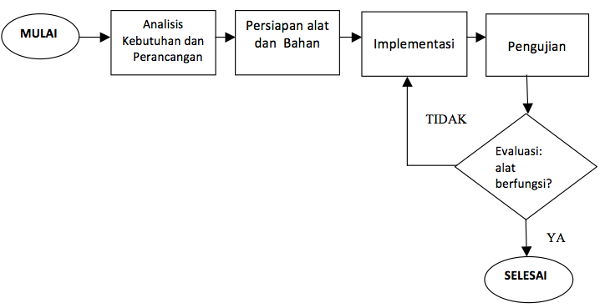
\includegraphics[width=200pt]{kolokium_contoh_gb1.png}
\caption{Tahapan proses penelitian}
\label{fig:tahapan}
\end{figure}
\fi
\subsection*{Analisa Kebutuhan dan Perancangan}

Komponen utama yang akan digunakan pada penelitian adalah komputer / laptop dengan dukungan OpenCV dan kamera digital. Gambar \ref{fig:alat} merupakan ilustrasi dari alat yang akan dibuat.

\begin{figure}[h!]\centering % Gunakan \begin{figure*} untuk memasukkan Gambar
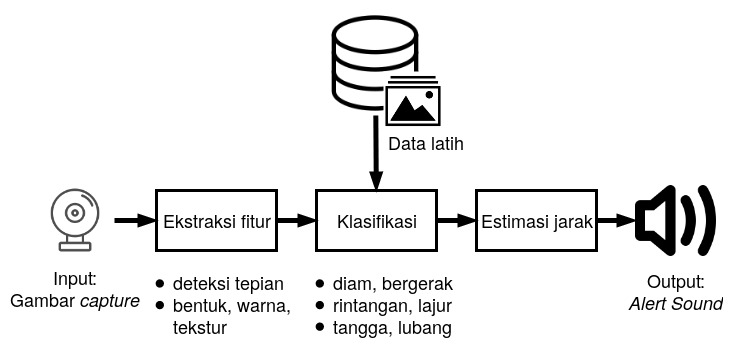
\includegraphics[width=\columnwidth]{prototipe-obstacle-detector}
\caption{Ilustrasi prototipe}
\label{fig:alat}
\end{figure}

\subsection*{Persiapan Alat dan Bahan}

Kegiatan yang dilakukan pada tahap ini adalah mengumpulkan alat dan bahan yang akan digunakan pada penelitian, yakni:
\begin{enumerate}
	\item Komputer dengan dukungan OpenCV dan C++
	\item Kamera portable yang dapat dikoneksikan dengan komputer untuk \textit{live video} atau dapat pula menggunakan file video yang direkam sebelumnya.
	\item Persiapan data latih yang akan digunakan untuk pengenalan objek dan klasifikasi. Pada tahapan ini software yang digunakan adalah RStudio.
\end{enumerate}

\subsection*{Implementasi}

Pada tahap ini dikembangkan produk berupa prototipe program berbasis C++ mennggunakan library OpenCV.

\subsection*{Pengujian dan Evaluasi}

Pengujian dilakukan untuk mengukur akurasi hasil pengenalan objek. Aplikasi berusaha:
\begin{enumerate}
	\item mendeteksi objek yang telah didefinisikan, di antaranya: pejalan kaki, kendaraan, dan pintu
	\item objek yang tidak dikenal dikategorikan menjadi objek diam, atau objek bergerak. 
	\item memperkirakan estimasi jarak dari posisi pengguna ke posisi objek.
	\item jangkauan deteksi adalah maksimal 10 meter di depan kamera.
	\item Output berupa \textit{tone} rendah dengan beberapa variasi frekuensi dan tempo untuk membedakan jenis objek dan estimasi jarak.
\end{enumerate}

\iffalse
\subsection*{Evaluasi}

Pengujian yang dilakukan di tahap sebelumnya dievaluasi pada tahap ini. Pengujian pertama dinyatakan berhasil jika efisiensi frekuensi mencapai 100$\%$ artinya frekuensi yang dihasilkan sesuai dengan input yang dimasukkan. Pengujian kedua dinyatakan berhasil jika tikus yang berada pada kandang berpindah tempat ke kandang lain setelah terkena gelombang ultrasonik dari alat. Pengulangan implementasi dilakukan jika salah satu atau kedua pengujian dinyatakan tidak berhasil atau gagal.
\fi
\subsection*{Jadwal Kegiatan}

Penelitian ini akan dilakukan dalam 5 pekan dengan rincian kegiatan seperti tercantum pada Tabel \ref{tab:jadwal}.
\begin{table}[t!]
	\begin{center}
		\caption{Rencana Jadwal Penelitian}
		\label{tab:jadwal}
		\footnotesize
		\begin{tabular}{|l|c|c|c|c|c|}
			\hline
			\iffalse
			\multirow{2}{*}{Kegiatan}&\multicolumn{2}{c|}{1}&\multicolumn{4}{c|}{2}&\multicolumn{4}{c|}{3}&\multicolumn{4}{c|}{4}&\multicolumn{4}{c|}{5}\\
			\cline{2-19}
			\fi
			Kegiatan&1&2&3&4&5\\
			\hline \hline
			Persiapan alat dan bahan &\cellcolor{black}&&&&\\
			\hline
			Penyusunan data latih&&\cellcolor{black}&\cellcolor{black}&&\\
			\hline
			Implementasi&&&\cellcolor{black}&\cellcolor{black}&\\
			\hline
			Pengujian dan Evaluasi&&&&\cellcolor{black}&\cellcolor{black}\\
			\hline
		\end{tabular}
		\normalsize
	\end{center}
\end{table}

\iffalse
\subsection*{Contoh Penulisan}

Bagian ini sengaja diisi dengan beberapa contoh penulisan dalam LaTex untuk memudahkan menulis makalah dengan cepat menggunakan LaTex. Berikut adalah contoh membuat tabel yang dapat dirujuk. Misalnya, Tabel \ref{tab:daftarsaya} menjelaskan sesuatu yang terkait dengan naskah ini.

\begin{table}[hbt]
\caption{Daftar Nilai}
\centering
\begin{tabular}{llr}
\toprule
\multicolumn{2}{c}{Name} \\
\cmidrule(r){1-2}
First name & Last Name & Grade \\
\midrule
John & Doe & $7.5$ \\
Richard & Miles & $2$ \\
\bottomrule
\end{tabular}
\label{tab:daftarsaya}
\end{table}

Kadangkala kita juga perlu menuliskan suatu formula matematika dalam sebuah kalimat. Misalnya, ada formula matematika $\cos^3 \theta =\frac{1}{4}\cos\theta+\frac{3}{4}\cos 3\theta$, dimana penulisan formula ini berbeda dengan formula sebelumnya yang diberi referensi atau nomor formula yang dapat diacu di dalam sebuah teks kalimat.

Tabel \ref{tab:tag} menunjukkan contoh suatu tabel yang memiliki lebar melebihi kolom yang diinginkan, sehingga perlu diatur lebar sesuai yang diinginkan. Dalam hal ini digunakan paket \textit{tabulary}.

\begin{table}[h!]
\footnotesize
\caption{Deskripsi dokumen XML tanaman obat}
\centering
\begin{tabulary}{0.45\textwidth}{LL}
\toprule
\parbox{12em}{Nama Tag} & Deskripsi \\
\midrule
$<$dok$>$&Mewakili keseluruhan dokumen\\
$<$id$>$&Menjelaskan id dokumen\\
$<$nama$>$&Nama tanaman obat\\
$<$namal$>$&Nama latin tanaman obat\\
$<$deskripsi$>$&Deskripsi tanaman obat yang terdiri dari manfaat, habitus, bagian yang digunakan dan kandungan zat kimia\\
$<$fam$>$&Famili tanaman obat\\
$<$penyakit$>$&Penyakit yang dapat disembuhkan oleh tanaman obat.\\
\bottomrule
\end{tabulary}
\label{tab:tag}
\end{table}

\subsection*{Contoh Penulisan Algoritme}
Algoritme \ref{algo:max} dibuat untuk mendapatkan bilangan terbesar dari kumpulan bilangan yang terhingga.

\begin{algorithm}
\DontPrintSemicolon % Some LaTeX compilers require you to use \dontprintsemicolon instead
\KwIn{Himpunan $A=\{a_1, a_2, \ldots, a_n\}$}
\KwOut{Bilangan terbesar}
$max \gets a_1$\;
\For{$i \gets 2$ \textbf{to} $n$} {
  \If{$a_i > max$} {
    $max \gets a_i$\;
  }
}
\Return{$max$}\;
\caption{{\sc Max} mendapatkan bilangan terbesar}
\label{algo:max}
\end{algorithm}
\fi